\section{Related work}
There are several existing HDI visualization tools that allows user to view the dataset in a non-interactive way. UNDP has a line chart(Figure \ref{fig:undp}) where the x axis is the year and y axis tis the HDI value.  Each line represent one country that user can hovers on to see specific value. It can be convenient if the user want to view the main trend for all countries or if the user want to find a country with highest or lowest HDI value through years. However, there is no much information they can retrieve from the middle range of data where many lines congested together. Also, it can be hard to find a specific country that looks interesting to the users. Another major visualization for HDI is Visualizing Human Development Index 2013 from Amazon AWS(Figure \ref{fig:amazon}), where it provides four line charts for HDI components and a color map that shows different HDI values. User is able to hover on the map or the line to see corresponding country highlighted. It also includes population chart for viewing how the population is distributed among different HDI values.  The comparison view between the map and the graph provides more information than the single line chart from UNDP. However, it didn't provides any filtering functionality if the user only want to view countries with high HDI. And it can be hard to find a country as well if the user doesn't know where the country is located on the map. For our visualization, we will try to provide user more opportunities to interact with the visualization so that they can easily find information they needed.
\begin{figure}[h!]
	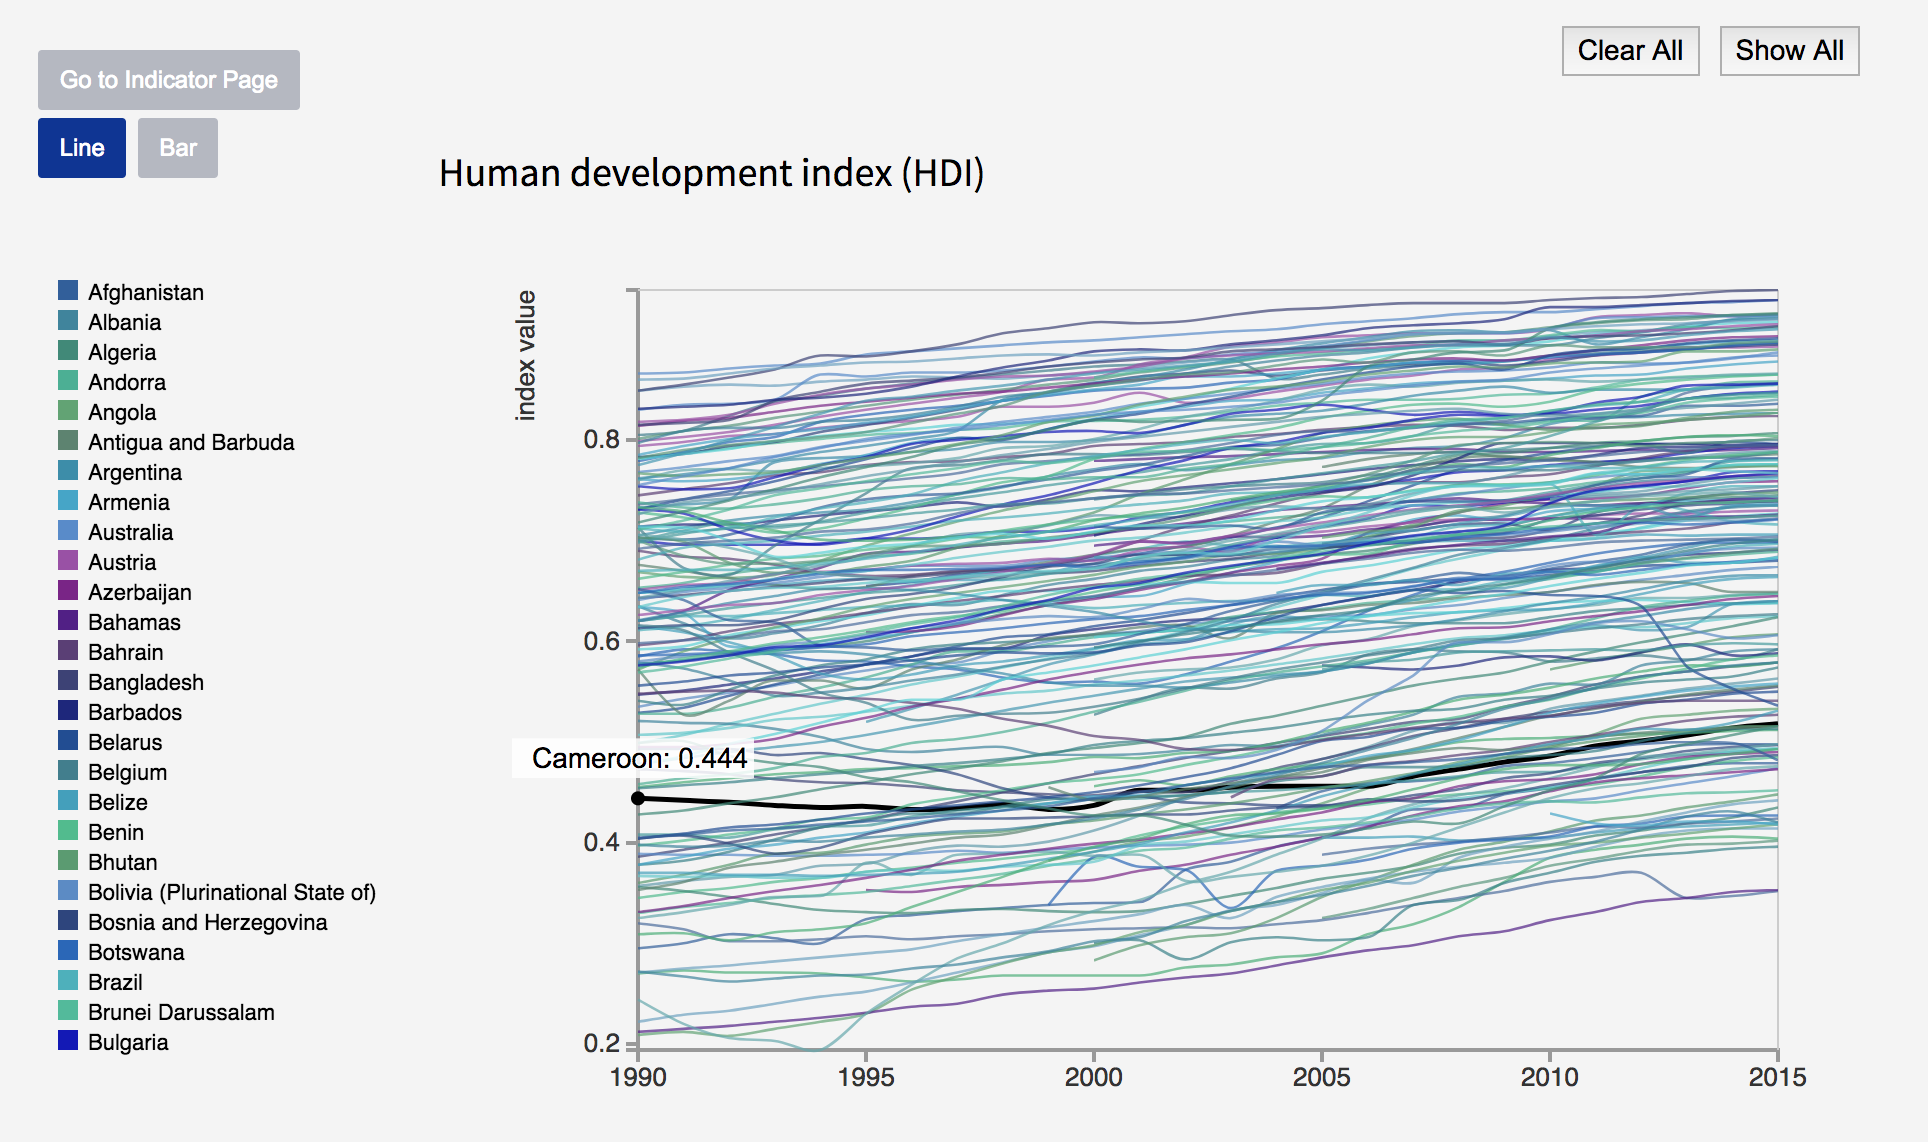
\includegraphics[width=0.4\textwidth]{undp}
	\caption{line chart map from UNDP}
	\label{fig:undp}
\end{figure}
\begin{figure}[h!]
	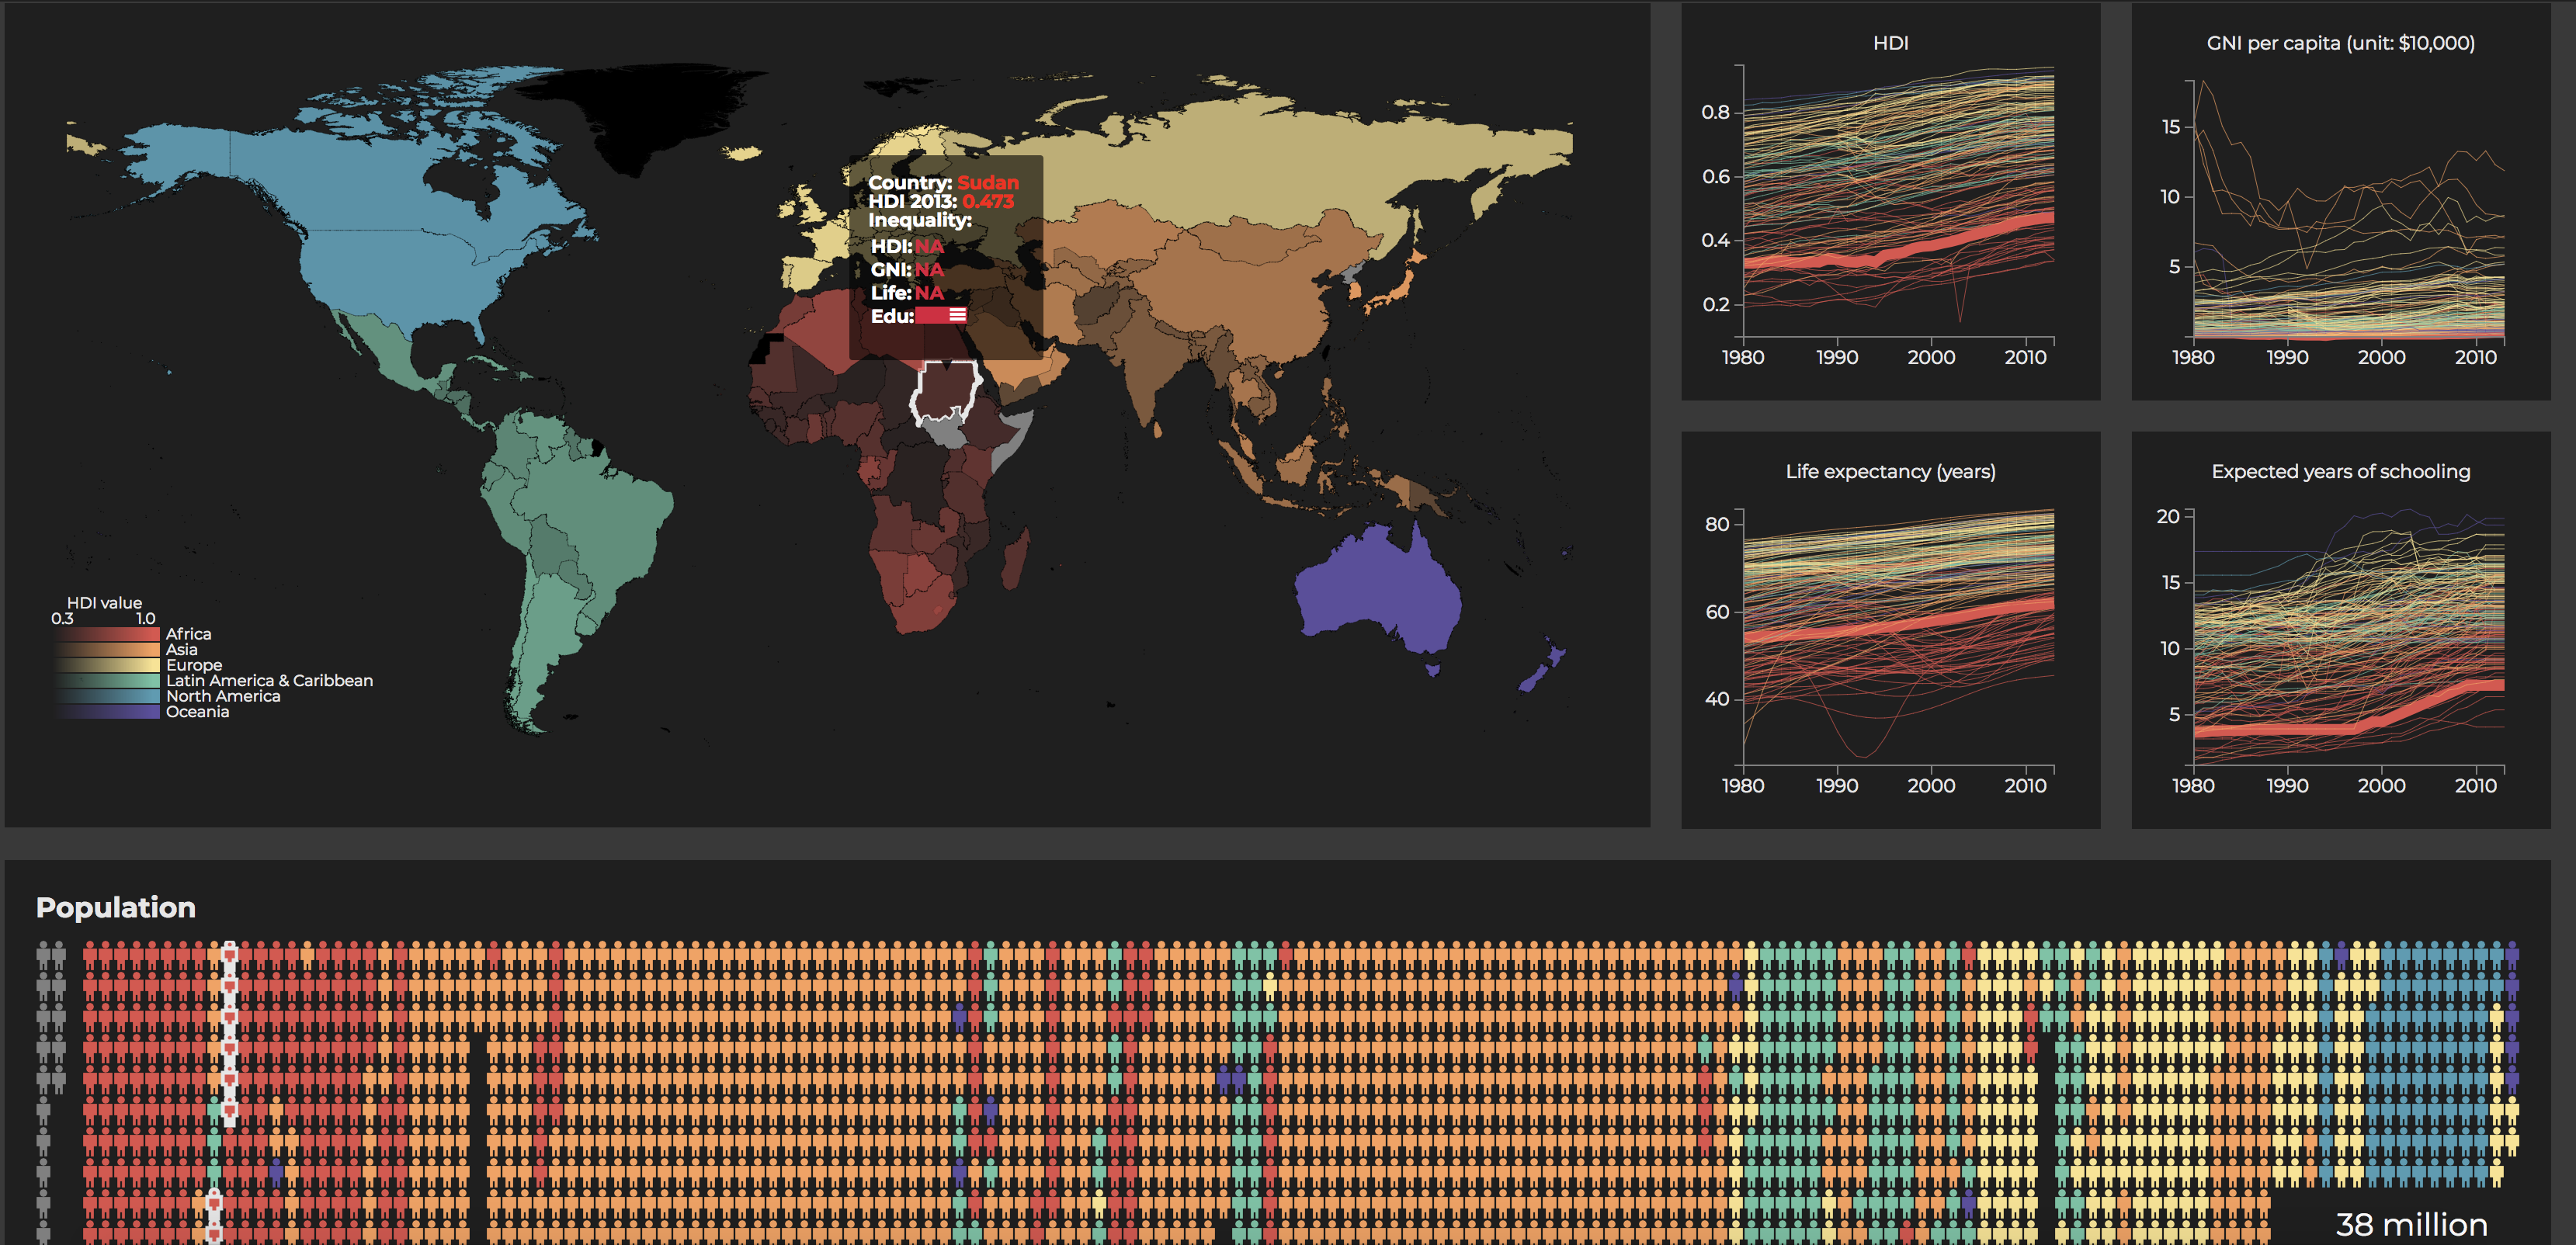
\includegraphics[width=0.4\textwidth]{amazon}
	\caption{Visualizing Human Development Index 2013}
	\label{fig:amazon}
\end{figure}
